\documentclass[12pt, a4paper, doc]{apa6}
\usepackage[american]{babel}
\usepackage{csquotes}
\usepackage[style=apa,sortcites=true,sorting=nyt,backend=biber]{biblatex}
\DeclareLanguageMapping{american}{american-apa}
\addbibresource{image_processing.bib}

\usepackage{graphicx}
\usepackage{fullpage}
\usepackage[parfill]{parskip}
\setlength{\parskip}{\baselineskip}
\usepackage{float}
\floatstyle{boxed}
\restylefloat{figure}
\usepackage{wrapfig}

\author{Richard Polzin, Studentnumber i6145946}
\affiliation{\today, Academic Writing, Tutor: Denise McAllister}
\title{Feature detection in the RoboCup SPL \\\ \large{An examination of the algorithms used by the 2016 world champion}}
\shorttitle{Feature detection in RoboCup}

\abstract{ This is the \textbf{Abstract.} Nice, huh ? }

\begin{document}
  \maketitle
  \setlength{\parindent}{0pt}

  \section{Introduction}
  \noindent 'By the middle of the 21st century, a team of fully autonomous humanoid robot soccer players shall win a soccer game, complying with the official rules of FIFA, against the winner of the most recent World Cup.', \cite{Kitano95robocup:the}. This is the official goal of the RoboCup initiative, an international scientific initiative which has several leagues and competition domains wherein robotic teams compete. In addition to competition against other teams, the physical setting of the challenges become more and more realistic year to year. Autonomous, programmable, humanoid robots called 'Nao' are used in the RoboCup Standard Platform League (SPL). A Nao V5 robot has a height of 58 cm and weighs 4.3 kg. It features an 1.6 GHz Intel Atom processor and 1 GB of RAM. The two legged robot is equipped with multiple sensors, as well as wifi, ethernet, and usb interfaces.

  In an attempt to make the environment of the game more realistic, the characteristics of the soccer field are changed regulary. For example, as in the 2008 RoboCup, navigation beacons were used to flag points of interest on the field. Furthermore, the field is no longer surrounded by walls and its size was increased to 60cm by 90cm. In the 2015 tournament, the goals were made color-neutral, whereas previously it was possible to differentiate goals by color.

  As the RoboCup competitors constanly try to keep up with the increasing difficulty of the game, different localization techniques have been investigated and researched. Localization refers to the task of autonomously tracking and maintaining an estimate of a robots location. It is critical for the robots to combine location estimation techniques to acertain a workable estimate. Some robots rely on ultrasonic sensors or lasers, and still others work with an electrical compass. The Nao robots include ultrasonic sensors as well as cameras. This paper will focus on image-based techniques.

  First of all the importance of image-based localization will be emphasized. Furthermore the concept of those techniques is explained. Then the obstacles that have to be overcome to provide a good localization are shown. The techniques of the B-Humon Nao team are then explained. Their important features are extracted and described. Finally the techniques evaluated.

  \section{Image-based Localization}
  In a game of soccer, where the robots need to react and collaborate quickly, localization is vital. Passing the ball, positioning, and dribbling all require fast and accurate localization. Localization can be split into local and global localization. Local localization focuses on objects distances relative to the robot. Questions arise and must be answered in very near real time. How far away are other players, goals, and walls? What is the distance to the wall? Answering these questions is integral to good play. On the other hand, global localization comes into play when a robot has to be removed from the field or is replaced. Maintaining the global position on the field allows for better positioning and general orientation, especially with the color coding of the goals removed. For high-quality play, it is important to keep track of the sites of the field. Having great dribbling and shooting many goals is not sufficient if the robot mixes up the enemy goal and its own.

    \begin{wrapfigure}{r}{0.5\textwidth}
      \begin{center}
        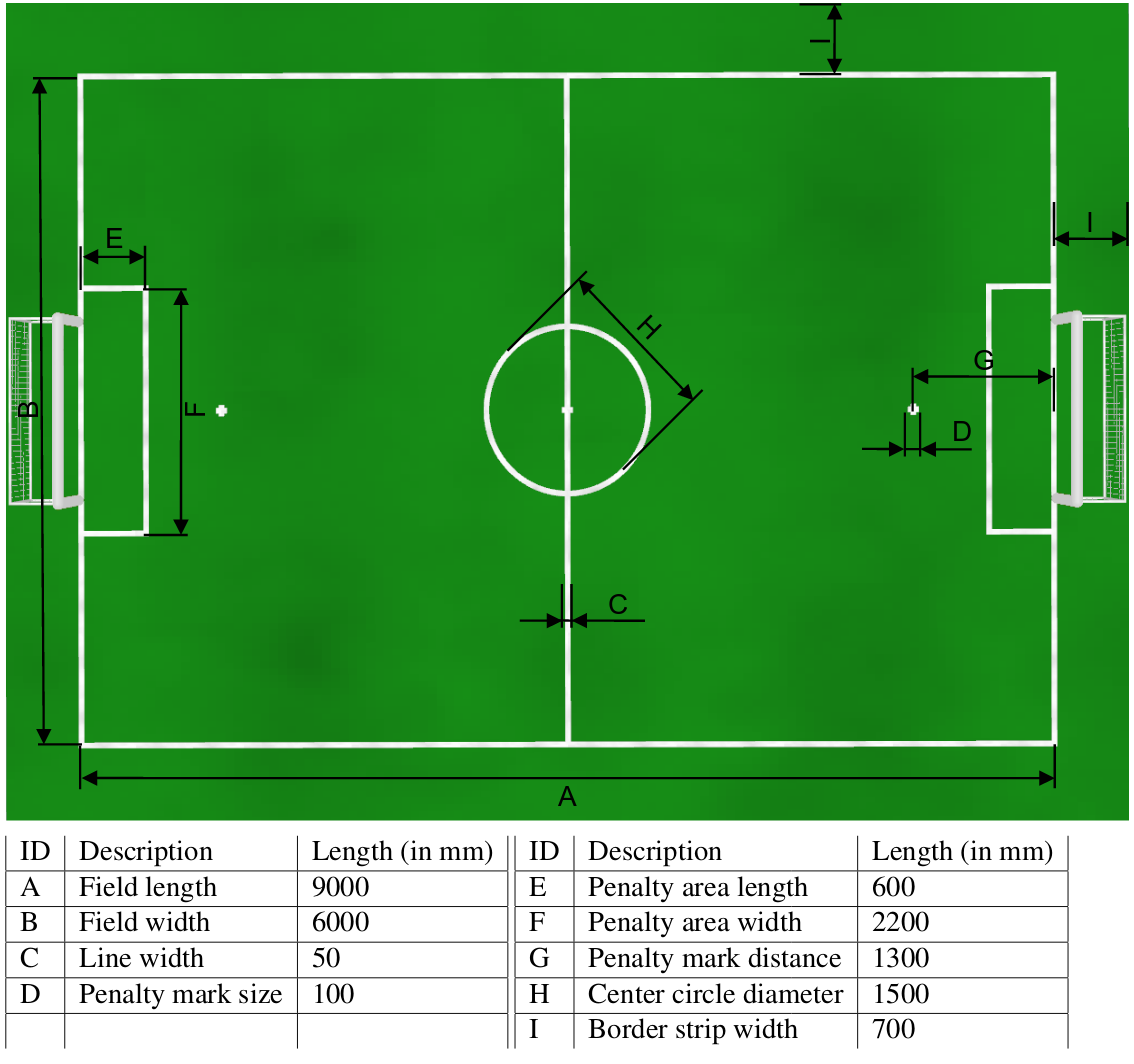
\includegraphics[width=0.48\textwidth]{field.png}
      \end{center}
      \caption{Schematic diagram of the soccer field based on rules stated by the \cite{soccerfield}}
    \end{wrapfigure}

  Localization of the Nao robot is only possible with the sensors it provides. \cite{naosheet}, offers documentation on the different sensors. The Nao offers microphones, tactile sensors, bumbers, four sonar sensors, and two cameras. Neither microphones, tactile sensors, nor bumpers are valuable to detect objects far away. Only the camera and sonar sensors can be used. The sonar sensors are divided in two receiving and two emitting devices. Detection was initially possible in the range 20 cm to 80 cm, but with the V4 Version of the Nao, detection range increased to 20 cm to 2.55 m. The camera sensors are positioned in the head and provide an image with 1280 x 960 pixels at 30 frames per second. Image [] show the orientation of the cameras, while the sonar sensors can certainly be used for collision avoidance and player / ball detection, the camera sensors are more often used for localization. This paper, as well as the different techniques explained later on, will not use the sonar senors, but only work with the cameras.

  After concluding that localization is important, and that cameras are the most promising sensors to use, the concept of image-based localization is explained. A good self-localization should be fast and reliable. Localization needs to run fast enough to react quickly to changes during play and still leave enoungh computational power for the other important algorithms. Furthermore, there should always be an solid estimate of the robots position and should be able to overcome the challenges described in detail in the next section. In general, such a localization process consists of three steps. First an image is recorded and some arbitrary feature is detected. For example the image is scanned for the rectangle of a goal. The second step creates an abstract model of the detected feature. A goal is perceived no longer as a flat rectangle, but as an 3D object. 3D position is determined, and the distance to the robot is calculated. In the final step the robots local map is positioned into the coordinate system of the whole soccer field. Based on the current vision of the robot and its distance to the goal the robots position on the soccer field is determined. The three steps must be individually well-executed and collectively accurate to achieve an optimal localization. Most papers published in the field of RoboCup SPL localization present techniques including all three steps, and adjust them according to a given strategy. Due to the limited scope of this paper, the comparison of techniques will focus on the first step: the extraction of physical geometric features from the image.

  \section{Challenges}
  Image-based localization in RoboCup SPL has to overcome several obstacles that are important in more practical robot applications as well. While the robots sensors are gradually improving year to year, the challenges they face increase as a increasing rate. Similar to human vision, the cameras on the Nao robots offer only a limited field of view. They have to move their heads to fully assess their environment and can't rely on powerful omnidirectional sensors. The cameras have to deal with different lighting conditions. While initially high-quality light was required by the rules, nowadays the game isn't interrupted, even when lightbulbs break down. Additionally, the earlier mentioned color codings were removed. Finally, photographers are now allowed to freely use flash.

  All these different aspects can lead to low quality pictures from the cameras. However, environmental factors are not alone in restricting image uptake quality. While shooting in RAW with a high-quality DSLR and post-processing the image would produce much better results, hardware shall not be changed, and thus hardware limitations must be considered. The 1.6 GHz of the Atom processor and the 1 GB of RAM are all the resources available. Computations still have to be executed as near to real-time as possible. Even ignoring image quality, there are still further challanges to face when it comes to localization. Robots can stand in each others way and occlude the field of view. Relying on color is dangerous as well, as the environment could become more noisy in the future. As the RoboCup initiative aims to win an official FIFA game with colorful advertisements, noisy chanting, and dramatic lighting, these challenges must be predicted and mitigated in localization implementations.

  In conclusion, there are many and varied challenges facing image-based localization which must be addressed to if the ultimate goal of beating a world-class human soccer team is to be achieved.

  \section{Overview of Techniques}
  Images [] show everything that defines the 2015 RoboCub SPL soccer field. It's a mostly-white field with lines and goals on a green carpet. The goal posts and crossbar are white, while the net and support structure can be white, gray or black. Lighting can only come from the ceiling and any changes in the lighting will not be cause for delay. Fields can be in visible range of one another, but if they are they must be at least three meters apart.

  The B-Human RoboCup team was founded in 2006 and started participating in the SPL in 2009. They competet in seven RoboCups and became world champion four times. Their code is available on GitHub with the intention of nurturing the scientific community and allowing teams who can't afford to develop a complete robot soccer system to participate. For localization the B-Human team uses 'field lines, their crossings, and the center circle' []. In 2015 they added support for penalty area detection. Those features are detected on an image, which in then used to conclude the robots possible positions. B-Human calls those features 'field features'. They include the features mentioned above and the goal frame on the floor.

  The images of the Nao's cameras are preprocessed to improve the results of the field feature extraction. [] states, that B-Human uses a color separation algorithm for this task. Due to the nature of the camera and the color space they record images in, detection of the color white is not trivial. The B-Human team solved this issue by detecting orange (the ball) and green (the field), deducing which parts of the field are probably white. This image is then used to detect the field features.

  Field lines are detected by collecting all regions that are 'line shaped'. Those are regions that are white and border on green regions. In the next step a greedy algorithm enlarges a line to some extend. Those combined lines are classified and verified for further processing. Verification includes for example an observation of the lines height, so that a robot that accidentally was detected as a part of a line would trigger an error. The classification takes place on the crossing points. They are classified as \emph{T} or \emph{L} crossings, depending on the connected lines. Finally lines are clustered to detect possible circles and linear regression is used to fit a center circle in those clusters. If the fitting error is small enough, the center circle was found.

  The penalty area detection was added in 2015 due to the removal of color coding on the goals. It was important to find another reliable area to compensate for that change. Due to the geometrical setup of the penalty area it is unique and therefor a good orientation. The goal's position can be approximated and even if the penalty point itself is obstructed, the rectangular area can be used as a reference.

  Due to the white color of the goals it has become harder to detect them. The background of the goals can be white as well, so that the borders can be blurred. White goals, white supports and white backgrounds rise new challenges in the goal detection algorithms. B-Human detects goals by searching for white regions directly below the field borders. The Rules state, that Robots and goal posts are the only white objects that can be present on the field. The referee is wearing dark blue or black clothing and the ball is orange. Knowing the size of a goal the image can be cropped to the approximate dimensions and processed further. The Sobel operator is used to create an image that emphasizes the edges. A Hough transform is then used to detect lines. All possible goal lines are fitted onto a model of the goal and if a certain threshold is met, a goal was detected.

  Combining the field features a model of the current field is constructed and mapped to the known dimensions of the field. In combination with probability theory and history tracking, this technique is used to localize the robot on the soccer field.

  \section{Conclusion}
  In this paper a general introduction to the RoboCub Standard Platform League was given. The challenges of this league have been discussed with a focus on localizing a robot on the soccer field. This aspect was further discussed and the task was broken down into three parts. The first part, feature extraction, was then analyzed in detail and the techniques used by the current world champion team, B-Human, were presented. The B-Human team uses color based separation to prepare the image for a grid-based region finding algorithm. Those regions are grouped and combined to determine field lines and crossing, the penalty area and the center circle. To detect the goals the Sobel operator is used in combination with a Hough transform to detect the edges and fit the goal to a model.
  The self localization of B-Human obviously is one of the best and some of the fundamental techniques used in the process were described in this paper. They are available in the B-Human framework, that can be used in the RoboCup competition and documented in their different publications.

\end{document}
